\section{Conway's Game of Life}
\begin{frame}{Conway's Game of Life}
    \LARGE
    \begin{center}
        Try to google: "Conway's Game of Life"
    \end{center}
\end{frame}

\begin{frame}{Overview of Conway's Game of Life}
\small
\begin{itemize}
    \item \textbf{Overview:}
    \begin{itemize}
        \item Created by the mathematician John Horton Conway in 1970.
        \item A zero-player game where evolution is determined by its initial state, without stochastic elements.
        \item The game unfolds on an infinite grid.
        \item Each cell can be either alive or dead.
    \end{itemize}
    
    \item \textbf{Rules of Evolution:}
    \begin{enumerate}
        \item Any live cell with fewer than two live neighbors dies.
        \item Any live cell with two or three live neighbors lives on to the next generation.
        \item Any live cell with more than three live neighbors dies.
        \item Any dead cell with exactly three live neighbors becomes a live cell.
    \end{enumerate}
\end{itemize}
\end{frame}

\begin{frame}{Each cell can be either alive or dead.}
    \vfill
    \begin{center}
    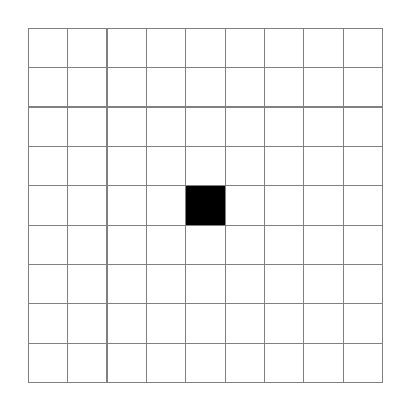
\begin{tikzpicture}[scale=0.5]
    \fill (4,4) rectangle (5,5);
    \draw[gray] (0,0) grid (9,9);
    \end{tikzpicture}
    \end{center}
\end{frame}

\begin{frame}{The status of each cell changes each generation.}
Status depends on the status of the cell and its 8 neighbors.
    \vfill
    \begin{center}
    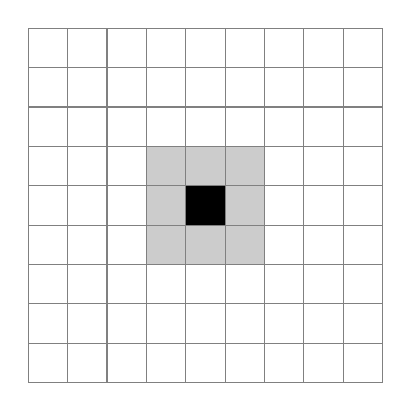
\begin{tikzpicture}[scale=0.5]
    \fill[gray!40] (3,3) rectangle (6,6);
    \fill(4,4) rectangle (5,5);
    \draw[gray] (0,0) grid (9,9);
    \end{tikzpicture}
    \end{center}
\end{frame}

\begin{frame}{At each step, transitions occur according to four rules}
\only<1-2>{\textbf{Rule 1:} Any live cell with fewer than two live neighbors dies, as if by underpopulation.}
\only<3-5>{\textbf{Rule 2:} Any live cell with two or three live neighbors lives on to the next generation.}
\only<6>{\textbf{Rule 3:} Any live cell with more than three live neighbors dies, as if by overpopulation.}
\only<7-8>{\textbf{Rule 4:} Any dead cell with exactly three live neighbors becomes a live cell, as if by reproduction.}
    \vfill
    \begin{center}
    \begin{tikzpicture}[scale=0.5]
    \only<1-2>{\fill (4,4) [secondary] rectangle (5,5);}
    \only<3-5>{\fill (4,4) [primary] rectangle (5,5);}
    \only<6>{\fill (4,4) [secondary] rectangle (5,5);}
    \only<8>{\draw[thick, blue, fill=primary!20] (4,4) rectangle (5,5);}
    \draw[gray] (0,0) grid (9,9);
    \fill (4.5,4.5) circle (3pt);
    \end{tikzpicture}
    \end{center}
\end{frame}

\begin{frame}{Frame Title}
    \Large
    \begin{center}
        Starting from the initial configuration, these rules are applied, and the game board evolves, playing the game by itself.
    \end{center}
\end{frame}

\begin{frame}{Example of pattern evolution}
  \begin{center}
    \begin{tikzpicture}[scale=0.5]
    \only<1>{
    \fill (5,5) rectangle (6,6);
    \fill (4,3) rectangle (5,5);}
    \draw[gray] (0,0) grid (9,9);

    \only<2>{
    \fill (5,5) [gray!30] rectangle (6,6);
    \fill (4,3) [gray!30] rectangle (5,5);
    \fill (4,4) rectangle (6,5);}

    \only<3>{
    \fill (5,5) [gray!30] rectangle (6,6);
    \fill (4,3) [gray!30] rectangle (5,5);
    \fill (4,4) [gray!30] rectangle (6,5);}
    \end{tikzpicture}
    \end{center}
\end{frame}

\begin{frame}{Oscillators}
Periodic Life Forms or Oscillators are life forms that oscillate periodically.
  \begin{center}
    \begin{tikzpicture}[scale=0.5]
    \only<1>{
    \fill (3,4) rectangle (6,5);
    }
 
    \only<2>{
    \fill (3,4) [gray!30] rectangle (6,5);
    \fill (4,3) rectangle (5,6);
    }

     \only<3>{
    \fill (4,3) [gray!30] rectangle (5,6);
    \fill (3,4) rectangle (6,5);
    }
    \draw[gray] (0,0) grid (9,9);

    \end{tikzpicture}
    \end{center}
\end{frame}


\begin{frame}{Still Life}
Still Life: a stable, finite, and nonempty pattern.
  \vfill
    \begin{center}
    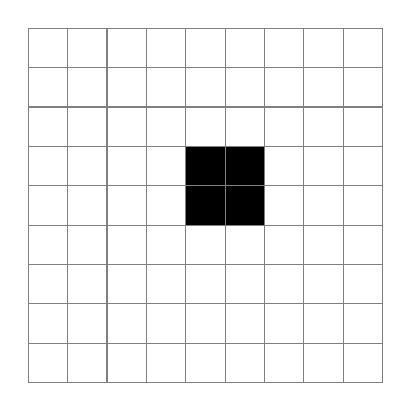
\begin{tikzpicture}[scale=0.5]
    \fill (4,4) rectangle (6,6);
    \draw[gray] (0,0) grid (9,9);
    \end{tikzpicture}
    \end{center}
\end{frame}

\begin{frame}{Glider}
A \textbf{glider} is a simple five-cell pattern that repeats itself every four generations and is offset diagonally by one cell. It is the smallest and most common type of spaceship. A spaceship is a pattern that moves across the game board.
  \vfill
    \begin{center}
    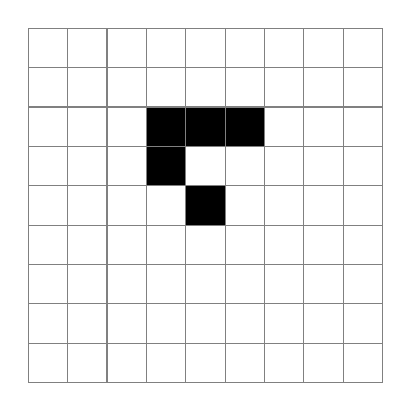
\begin{tikzpicture}[scale=0.5]
    \fill (3,5) rectangle (4,7);
    \fill (4,6) rectangle (6,7);
    \fill (4,4) rectangle (5,5);
    \draw[gray] (0,0) grid (9,9);
    \end{tikzpicture}
    \end{center}
\end{frame}

\begin{frame}{Some Patterns in Conway's Game of Life}
\small
\begin{itemize} 
    \item \textbf{\href{https://playgameoflife.com/lexicon/stillater}{Oscillators}:} Patterns that return to their initial state after a certain number of generations. 
    \item \textbf{\href{https://playgameoflife.com/lexicon/56P6H1V0}{Spaceships}:} Patterns that translate themselves across the board. 
    \item \textbf{\href{https://playgameoflife.com/lexicon/Garden_of_Eden_(1)}{Gardens of Eden:}} Configurations that cannot be reached from any other, meaning they have no predecessors.
    \item \textbf{\href{https://playgameoflife.com/lexicon/acorn}{Methuselahs:}} Start with a small configuration and evolve over many generations before stabilizing.
    \item \textbf{\href{https://playgameoflife.com/lexicon/eater1_(2)}{Eaters:}} Stationary or oscillating patterns that can destroy other patterns. Used to 'eat' gliders and other spaceships.
    \item \textbf{\href{https://playgameoflife.com/lexicon/backrake}{Rakes}:} Patterns that move like spaceships but also emit other patterns, typically gliders.
    \item \textbf{\href{https://playgameoflife.com/lexicon/Gosper_glider_gun}{Guns:}} Stationary patterns that periodically emit spaceships or other patterns.
    \item \textbf{\href{https://playgameoflife.com/lexicon/memory_cell}{Memory Cell:}} Stores information that can be read out.
\end{itemize}
\end{frame}

\begin{frame}
\frametitle{Constructing Logical Gates in Conway's Game of Life}
\begin{itemize}
    \item \textbf{Computational Universality:} Conway's Game of Life is Turing complete, meaning it can simulate a universal constructor or any Turing machine.
    \item \textbf{Logic Gates:} Using gliders and eaters, specific logic gates like AND, OR, NOT can be constructed.
    \begin{itemize}
        \item \textbf{AND Gate:} Two gliders collide in a way that if both are present, a new glider is formed (output).
        \item \textbf{OR Gate:} Gliders are sent such that if at least one arrives, a new glider is formed.
        \item \textbf{NOT Gate:} Utilizes a glider stream that is blocked unless another glider interferes, allowing a glider to pass through if no input glider is present.
    \end{itemize}
    \item \textbf{Application:} These gates can be used to build more complex circuits and perform computations.
    \item A computer with memory, a processor, and a display can be built in Conway's Game of Life.
\end{itemize}
\end{frame}

\begin{frame}{Task: How Will This Pattern Evolve?}
\begin{itemize}
    \item It is \textbf{impossible} to predict, in advance, what behavior will be displayed by the Cellular Automata given a set of rules.
    \item We will find out how the following shape evolves in the exercise.
\end{itemize}
  \vfill
    \begin{center}
    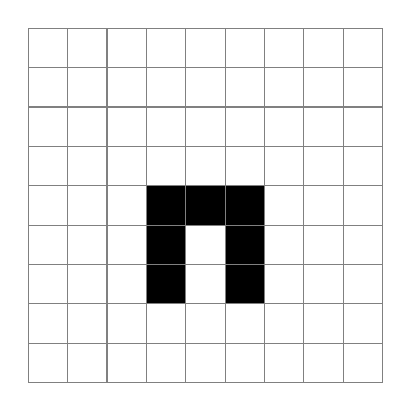
\begin{tikzpicture}[scale=0.5]
    \fill (4,4) rectangle (5,5);
    \fill (3,2) rectangle (4,5);
    \fill (5,2) rectangle (6,5);
    \draw[gray] (0,0) grid (9,9);
    \end{tikzpicture}
    \end{center}
\end{frame}
